\documentclass[onecolumn, draftclsnofoot,10pt]{IEEEtran}
\usepackage{graphicx}
\usepackage{url}
\usepackage{setspace}

\usepackage{geometry}
\usepackage{float}
\geometry{textheight=9.5in, textwidth=7in}

% 1. Fill in these details
\def \CapstoneTeamName{		    Team 42}
\def \CapstoneTeamNumber{		42}
\def \GroupMemberOne{			Michael Burton}
\def \GroupMemberTwo{			Rajat Kulkarni}
\def \GroupMemberThree{			Logan Saso}
\def \GroupMemberFour{			Miao Zhou}
\def \CapstoneProjectName{		Autonomous RC Car}
%\def \CapstoneSponsorCompany{	}
\def \CapstoneSponsorPerson{	D. Kevin McGrath}

% 2. Uncomment the appropriate line belofw so that the document type works
\def \DocType{	Requirement Document
				%Requirements Document
				%Technology Review
				%Design Document
				%Progress Report
				}
			
\newcommand{\NameSigPair}[1]{\par
\makebox[2.75in][r]{#1} \hfil 	\makebox[3.25in]{\makebox[2.25in]{\hrulefill} \hfill		\makebox[.75in]{\hrulefill}}
\par\vspace{-12pt} \textit{\tiny\noindent
\makebox[2.75in]{} \hfil		\makebox[3.25in]{\makebox[2.25in][r]{Signature} \hfill	\makebox[.75in][r]{Date}}}}
% 3. If the document is not to be signed, uncomment the RENEWcommand below
\renewcommand{\NameSigPair}[1]{#1}

%%%%%%%%%%%%%%%%%%%%%%%%%%%%%%%%%%%%%%%
\begin{document}
\begin{titlepage}
    \pagenumbering{gobble}
    \begin{singlespace}
        \hfill 
        % 4. If you have a logo, use this includegraphics command to put it on the coversheet.
        %\includegraphics[height=4cm]{CompanyLogo}   
        \par\vspace{.2in}
        \centering
        \scshape{
            \huge CS Capstone \DocType \par
            {\large\today}\par
            \vspace{.5in}
            \textbf{\Huge\CapstoneProjectName}\par
            \vfill
            {\large Prepared for}\par
            \Huge \CapstoneSponsorCompany\par
            \vspace{5pt}
            {\Large\NameSigPair{\CapstoneSponsorPerson}\par}
            {\large Prepared by }\par
            SmartRC\par
            % 5. comment out the line below this one if you do not wish to name your team
            %\CapstoneTeamName\par 
            \vspace{5pt}
            {\Large
                \NameSigPair{\GroupMemberOne}\par
                \NameSigPair{\GroupMemberTwo}\par
                \NameSigPair{\GroupMemberThree}\par
                \NameSigPair{\GroupMemberFour}\par
            }
            \vspace{20pt}
        }
        \begin{abstract}
        % 6. Fill in your abstract   
        This project has been created to pressure-test the potential mishandles and abuse that could be subjected to self-driving vehicles. The platform will consist of various sensors including Lidar, Ultrasonic, and Optical sensors to support testing various companies' implementations at a miniature level. Once the car is functional, tests will be run to measure the adaptability of the system to arbitrary environments including but not limited to, rough terrain, moving obstacles, and unseen or unreachable destinations. Many factors will contribute to the viability of the platform as a whole with passenger safety as a main concern. 
        \end{abstract}     
    \end{singlespace}
\end{titlepage}
\newpage
\pagenumbering{arabic}
\tableofcontents

\clearpage



\section{Introduction}
    The autonomous RC car will utilize a variety of different hardware components, such as sensors and a Nvidia Autonomy-Designed Computer. In terms of software, it will also include common machine learning libraries like OpenCV and Tensorflow w/ Keras. 
    
    Some key constraints include: 
    \begin{itemize}
        \item The car must safely avoid sizeable obstacles while driving over smaller ones;
        \item The car must be able to follow a certain path laid out by the user;
        \item The car must not require any human interaction whatsoever to complete the given path
    \end{itemize}

\subsection{Purpose}
    This project is intended to create an autonomous RC car that can travel between predetermined points A and B and back to A while avoiding any stationary or moving obstacles in an arbitrary environment.
\bigskip

\subsection{Intended use}
    The use of this platform is to identify, study, and rectify potential faults in autonomous vehicles. This allows for a scale-model study of worst-case situations an autonomous vehicle may encounter. For example, how could malicious actors influence the direction of the car for illicit purposes. It could also be used to test worst-case environmental scenarios such as bad routing or obstacle avoidance.
\bigskip

\subsection{Scope}
    The scope of work for this project is to create a unified system that links together multiple machine learning / self driving car technologies to create a unified platform that allows a research to configure the platform for testing. Some companies, like NVIDIA (the manufacturer of the brain in our system) provide object detection libraries for optical recognition, but don't expand that to LIDAR, Ultrasonic, or other detection methods. The platform will let the researcher configure which sensors and technologies are used to test them in different scenarios.
\bigskip

\section{Functional Requirements}

\bigskip

\subsection{Hardware}

\bigskip

\subsubsection{Sensors}
    The platform will utilize a combination of Lidar, Ultrasonic, and Optical sensors for obstacle detection and route planning. Firstly, Lidar will be serving as the short-range, high-accuracy sensor. This will help the platform make fine-grained judgments about its capabilities at the close range. For example, the car may not be able to tell from a distance if a particular rock is scalable, but when approaching it could use the Lidar to determine height, depth, or incline of the rock, and determine if its something it can drive over. Next, we will use Ultrasonic sensors for mid-range detection of rough objects. For example, Ultrasonic could help identify walls, cars, or significant path blockers.  Lastly, we will be using Optical Sensors, which is the longest range sensor on the platform. This sensor should be able to be the only functioning sensor and still have the platform work, as it’s capable of both long-range and short-range interpolation. It’s important that the system is able to switch between different sensors as required. It is important to note that companies that specialize in building autonomous vehicles use different sensors. For instance, Tesla does not rely on  Lidar to identify objects in the path, but rather Optical. The goal is to test different implementations of object avoidance, which means mixing and matching the specifications of different companies' implementations. 

\subsubsection{Car Body}
    The car body provided is sturdy and has sufficient space to mount various objects, such as the Lidar units, Optical sensors, and Nvidia unit. It's been modified to provide a suitable flat surface for mounting different sensors. Aesthetics are not a goal of this project.
    
    The Car we're using is a Traxxas Summit (pictured below) which comes with remote differential locking and a dual-speed transmissions. This in turn provides 4WD and combined with long-travel suspension lets the car scale objects nearly as tall as itself. It's important to note that the system should understand that certain objects, while scalable, might still be easier to go around. Some objects could be scaled, but we'd want to avoid animals or other moving objects. 
    
\begin{figure}[h!]
  \centering
  \textbf{Traxxis Summit Body}\par\medskip
    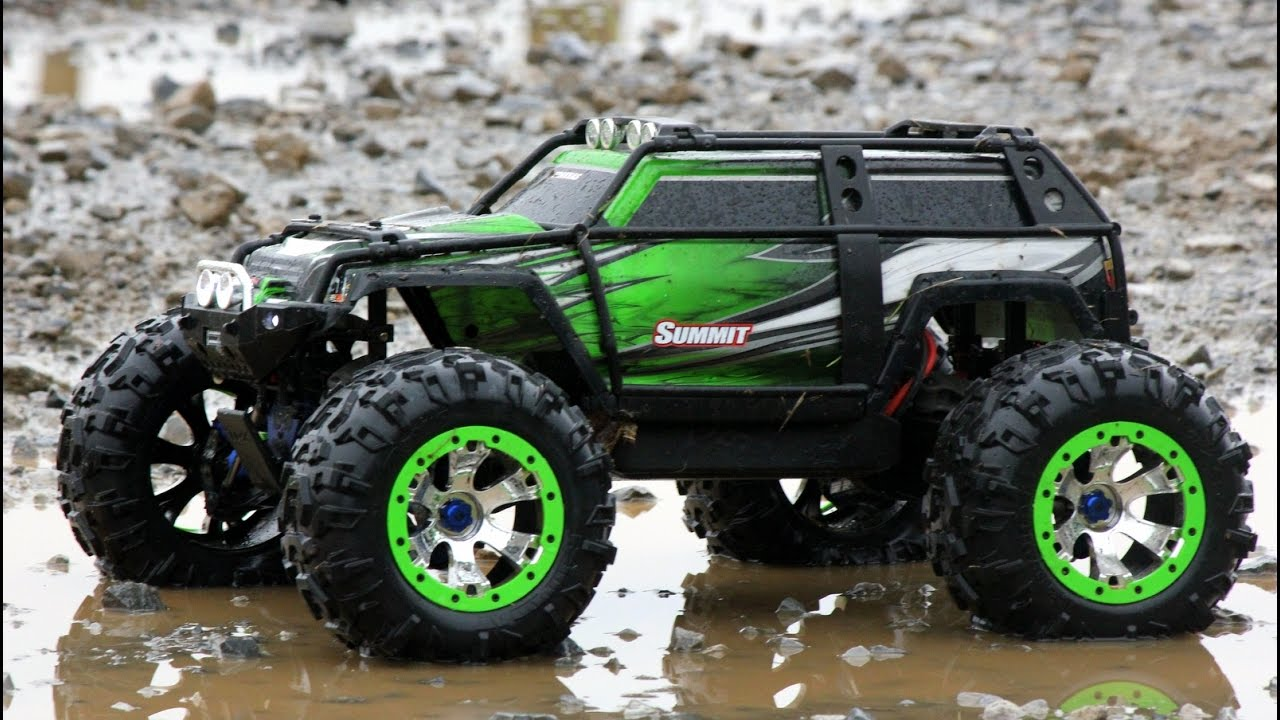
\includegraphics[width=\linewidth]{Summit.jpg}
    \caption{Traxxas Summit}
\end{figure}
 

    


\subsubsection{NVIDIA AGX Xavier}
    In order to implement the use of artificial intelligence for our autonomous vehicle, we will be using the NVIDIA Jetson AGX Xavier to provide us with the processing power that is necessary for our project. The Xavier is loaded with AI tools like NVIDIA Jetpack and DeapStream SDKs, as well as TensorRT. TensorRT is one of the main tools that will be used to provide the driving, routing, and avoiding capabilities as it comes pre-configured with Obstacle Detection and Image Classification networks. Obstacle Detection will be one of the primary uses of TensorRT for this project.
\bigskip

\subsection{Software}

    Languages:
    
    \begin{itemize}
    \item Rust
    \item C (where Rust is insufficient)
    \item Python
    \end{itemize}
    
  \noindent Libraries:
    
    \begin{itemize}
    \item OpenCV
    \item TensorFlow
    \item TensorRT
    \item DeepStream
    \end{itemize}
    
    \bigskip

    \noindent Overall, the software should be able to implement accurate environmental \textit{perception} and \textit{localization}; in other words, it should ensure that the car is able to process and categorize data by their "semantic meaning;" this includes small obstacles, pedestrians and animals. Localization entails that the car is able to determine where it is with respect to these obstructions. Furthermore, at a higher level, the software should ensure that the car is able to properly generate a series of steps (i.e. \textit{plan}) to achieve the overarching goal - which is primarily to safely maneuver from the start point, hit all the adjacent nodes, to the end point.[1]

\bigskip

\section{Nonfunctional Requirements}

\bigskip

\subsection{Safety}
    The hardware components of this project are very expensive, which presents us with having to make sure the vehicle has the proper safety measures in place. The vehicle will need to have a manual control switch that will immediately override the autonomous mode and give full control to the physical controller. This will ensure that if anything is to go badly, we will be able to correct it. It is also very important that we ensure the vehicle will not flip or collide while running; one way to do this is to limit the weight of materials mounted on top of the car body. By doing so, the risk of tipping over while making sharp turns will be mitigated. One of the most important features of autonomous vehicles is accident avoidance. Considering the cost of the parts we will be using, it is important to implement accident and obstacle avoidance as soon into the project as possible. 
    
\subsection{Quality}
    The overall quality of the car should be very high; it should manage to avoid all the right obstacles while scaling the proper ones; it should be able to follow a designated path; it shouldn't require any human interaction. Our system's quality will be judged with multiple tests. The vehicle will be tested on how quickly it can recognize a potentially hazardous situation and avoid it. For example, can the car avoid an oncoming vehicle at speeds of 10MPH, 20MPH, or 30MPH. Another quality test will be seeing how well the vehicle can navigate an environment filled with many different dynamic, and static obstacles. The vehicle will also be required to be able to correctly navigate to a given GPS location, or correctly say that it cannot reach that destination and return to start. In order for obstacle avoidance to be of quality, the car will need to be able to correctly judge what obstacles are able to be run over and which ones need to be avoided. Lastly, the visual quality of the car is not important.
    
\subsection{Security}
    While this platform in and of itself doesn't require a locked-tight security system, it's important to note that self-driving vehicles may be especially prone to theft. Particularly, self-driving cars have the capacity to be stolen remotely through the internet, as many if not all of them have a form of over the air updates. This means that, with the right exploit, hackers could tell your car to leave your house or they could simply walk up to it with the right device and unlock it. Our project does have the requirement that the self-driving mode can be remotely deactivated. This is important in situations where the self-driving capabilities fail or misjudge an obstacle. Note, though, that this project also expects the car to be capable of driving itself back to its launching point if it loses signal with the remote. Additionally, the car should be able to tell when its attempts at movement are failing, in the case that it flips over.
    
\subsection{Code Quality Concerns}
    As is the case for all self-driving vehicles, the quality of the platform is critical. When a piece of software encounters a bug it's typical to either log the bug and restart from a last-known success state or completely close the program. Unfortunately, neither of those are an option in the case of a self-driving car. In the first case, the last successful state of the vehicle is dependent on the sensor readings, so we can't simply "rewind" and try again, as time is always a factor. The second state isn't as much of a problem for a small RC car. If we want, we can set it up so that the car will automatically stop when encountering a critical fault. In a real car, though, this is an unacceptable state to be in. If we think of a real-life highway situation, it becomes clear that this behavior could very easily result in an accident causing potential injuries of the riders of all involved parties. For the lowest level interface with sensors, we propose that Rust be the programming language of choice. This is due to the fact that it is compiled, like C, has no runtime, like C, integrates very well with C interfaces where needed, but also performs static lifetime checking ensuring memory cleanup and thread safety. In Rust, there's no simple way to introduce a race condition or a null pointer deference, bugs which in the past have been responsible for deaths and serious loss of resources.
    
\bigskip

\subsection{Cost}
The maximum cost of the system is \$7000, including the RC car, onboard computer, and all required sensors. There will be no additional necessary costs.


\section{Project Timeline Prediction}
The following chart provides a layout and a timeline for our project this year.
\begin{figure}[H]
  \centering
   \textbf{Automated Traxxas Summit Gantt Chart}\par\medskip
    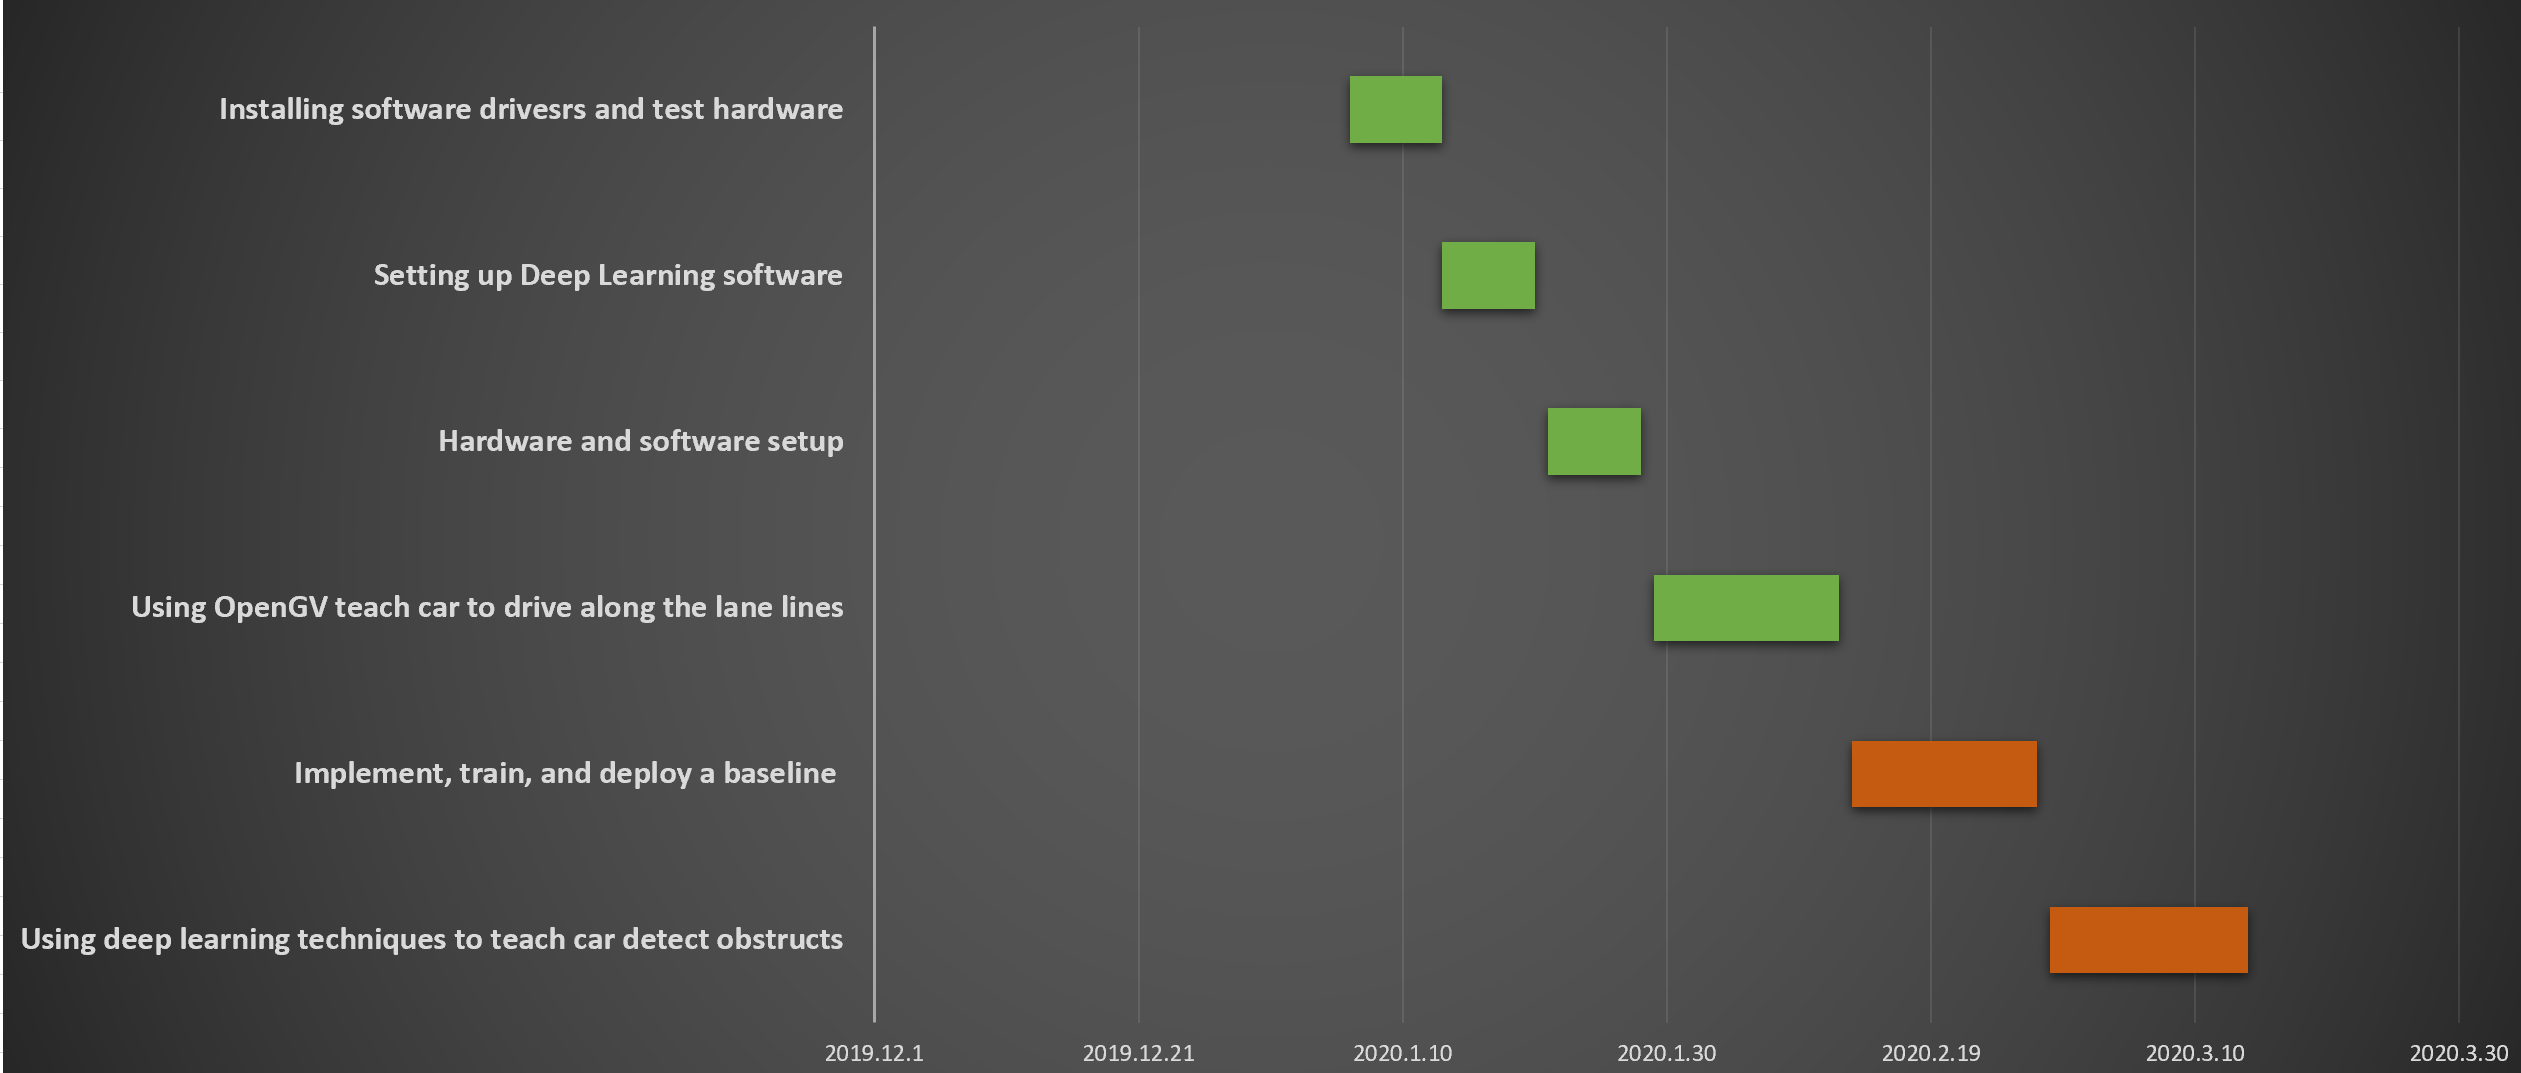
\includegraphics[width=\linewidth]{gantt.png}
    \caption{Gantt Chart}
\end{figure}

\bigskip
\bigskip
\bigskip

\begin{thebibliography}{99}

\bibitem{c1}Ang, Marcelo H. “Perception, Planning, Control, and Coordination for Autonomous Vehicles.” MDPI, Multidisciplinary Digital Publishing Institute, 17 Feb. 2017, https://www.mdpi.com/2075-1702/5/1/6/htm.

\end{thebibliography}

\end{document}